\documentclass{beamer}

\usepackage[T1]{fontenc}
\usepackage[utf8]{inputenc}

%\mode<presentation>{%
%  \usetheme{uvsq}
%}
\renewcommand{\emph}[1]{}
\usepackage{amsmath,amssymb,amsthm,multirow,algorithmic,graphics,color,ifpdf}
\usepackage{algorithmic,graphicx,tikz,pgflibraryarrows,pgflibraryplotmarks,pgflibrarysnakes,pgflibraryshapes}
\usepackage[section]{algorithm}
%\usepackage[matrix,arrow]{xypic}
%\usepackage{fullpage}
\newcommand{\C}{\mathbb{C}}
\newcommand{\R}{\mathbb{R}}
\newcommand{\Z}{\mathbb{Z}}
\newcommand{\N}{\mathbb{N}}
\newcommand{\Q}{\mathbb{Q}}
\newcommand{\F}{\mathbb{F}}
\newcommand{\KP}{\textbf{KP}}
\newcommand{\OW}{\textbf{OW-CPA}}
\newcommand{\INDCPA}{{\textbf{IND-CPA}}}
\newcommand{\INDCCA}{{\textbf{IND-CCA}}}
\newcommand{\INDCCATWO}{{\textbf{IND-CCA2}}}
\newcommand{\A}{\mathcal{A}}
\newcommand{\B}{\mathcal{B}}
\newcommand{\D}{\mathcal{D}}
\newcommand{\E}{\mathcal{E}}
\renewcommand{\c}{\mathcal{C}}
\newcommand{\G}{\mathcal{G}}
\newcommand{\I}{\mathfrak{I}}
\renewcommand{\O}{\mathcal{O}}
\newcommand{\p}{\mathfrak{p}}
\renewcommand{\P}{\mathcal{P}}
\newcommand{\iso}{\cong}
\newcommand{\stacksum}[2]{\genfrac{}{}{0pt}{}{{#1}}{{#2}}} %\substack is better
\newcommand{\jacobi}[2]{{\genfrac{(}{)}{}{}{#1}{#2}}}
\newcommand{\ord}{\operatorname{ord}}
\newcommand{\Res}{\operatorname{Res}}
%\renewcommand{\div}{\operatorname{div}}
\newcommand{\ndiv}{\nmid}
\renewcommand{\div}{\mid}
\newcommand{\Div}{\operatorname{div}}
\newcommand{\Pic}{\operatorname{Pic}}
\newcommand{\End}{\operatorname{End}}
\newcommand{\Cl}{\operatorname{Cl}}
\newcommand{\QR}{\operatorname{QR}}
\newcommand{\QNR}{\overline{\operatorname{QR}}}
\newcommand{\<}{\langle}
\renewcommand{\>}{\rangle}
\newcommand{\union}{\cup}
\newcommand{\intersection}{\cap}
\newcommand{\chr}{\operatorname{char}}
\newcommand{\id}{\operatorname{id}}
\newcommand{\Enc}{\operatorname{Encrypt}}
\newcommand{\Dec}{\operatorname{Decrypt}}
\newcommand{\pub}{{\operatorname{pubkey}}}
\newcommand{\priv}{{\operatorname{privkey}}}
\newcommand{\dlog}{{\operatorname{DLOG}}}
\newcommand{\cdh}{{\operatorname{CDH}}}
\newcommand{\ddh}{{\operatorname{DDH}}}
\newcommand{\bdh}{{\operatorname{BDH}}}
\newcommand{\dbdh}{{\operatorname{DBDH}}}
\newcommand{\LSB}{{\operatorname{LSB}}}
\newcommand{\MSB}{{\operatorname{MSB}}}
\newcommand{\Gal}{{\operatorname{Gal}}}
\renewcommand{\Pr}{{\operatorname{Prob}}}
\newcommand{\lcm}{{\operatorname{lcm}}}
\newcommand{\SL}{{\operatorname{SL}}}
\newcommand{\PSL}{{\operatorname{PSL}}}
\newcommand{\GL}{{\operatorname{GL}}}
\newcommand{\Ell}{{\operatorname{Ell}}}
\renewcommand{\a}{{\mathfrak{a}}}
\renewcommand{\b}{{\mathfrak{b}}}
\renewcommand{\L}{{\mathfrak{L}}}
\newcommand{\ignore}[1]{}
\renewcommand{\algorithmicrequire}{\textbf{Given:}}
\newcommand{\st}{\mid}
\newcommand{\eps}{\varepsilon}
\newcommand{\DL}{\operatorname{DL}}
\newcommand{\CDH}{\operatorname{DH}}
\newcommand{\PI}{\operatorname{PI}}
\newcommand{\BDH}{\operatorname{BDH}}
\newcommand{\IDH}{\operatorname{IDH}}
\newcommand{\IBDH}{\operatorname{IBDH}}

\newlength{\algcwidth} \newlength{\algcheight}
\newcommand{\algc}[1]{%
\settowidth{\algcwidth}{#1} \settoheight{\algcheight}{#1}%
\raisebox{1.2\algcheight}[0pt]{%
\makebox[0pt][l]{\hspace{.4\algcwidth}%
\rule{.6\algcwidth}{0.05\algcheight}}}%
{{#1}}}

\newcommand{\includeonlyiflecture}[1]{#1}
\newcommand{\includeonlyifbook}[1]{}

\newcommand{\cyc}[1]{{\langle #1 \rangle}}
\newcommand{\red}[1]{\textcolor{red}{#1}}
\newcommand{\blue}[1]{\textcolor[rgb]{0.24,0.15,0.70}{#1}}
\newcommand{\green}[1]{\textcolor[rgb]{0,0.8,0}{#1}}
\newcommand{\pink}[1]{\textcolor[rgb]{1,0.2,0.6}{#1}}
\newcommand{\orange}[1]{\textcolor[rgb]{1,0.6,0}{#1}}
\newcommand{\purple}[1]{\textcolor[rgb]{0.4,0.2,0.8}{#1}}

\usetikzlibrary{matrix,decorations}

\pgfkeys{/triangle/.code=\tikzset{x={(-0.5cm,-0.866cm)},y={(1cm,0cm)}}}

% This command defines a triangle of dots of given height
\newcommand{\dottriangle}[2][\i-\j]{%
  \foreach \i in {0,...,#2} {%
    \foreach \j in {0,...,\i} {%
      \draw(\i,\j) node{#1};%
    }%
  }}


\title{Yet another cryptosystem based on isogenies}
\author[Luca De Feo]{Luca De Feo\footnotemark[1]\\
  joint work with David Jao\footnotemark[2] and Jérôme Plût\footnotemark[1]}
\date[Montpellier, February 29, 2012]{February 29, 2012, Groupe de travail ARITH,\\
  LIRMM, Université de Montpellier 2}
\institute[UVSQ]{\footnotemark[1]Université de Versailles -- Saint-Quentin-en-Yvelines,\\
  \footnotemark[2]University of Waterloo}

\begin{document}

\frame{\titlepage}

%%

\begin{frame}
  \frametitle{Elliptic curves}

  As long as we are concerned in this talk, \emph{elliptic curves} are

  \begin{itemize}
  \item Algebraic \alert{groups} defined over a (finite) field.
  \item Their group law is easy to compute (say, in constant time).
  \item Any curve $E$ is (almost) uniquely defined by its
    \alert{$j$-invariant} $j(E)$ up to isomorphism (just a change of
    coordinates).
  \end{itemize}
  
  \[E \;:\; y^2 = x^3 + ax + b \qquad a,b\in k\]

  \alert{\[j(E) = 1728\frac{4a^3}{4a^3+27b^2}\]}
  
\end{frame}

%%

\begin{frame}
  \frametitle{Isogenies}

  Isogenies are just \alert{the right notion of morphism} for elliptic
  curves

  \begin{itemize}
  \item Surjective group morphism.
  \item Algebraic map (i.e., defined by polynomials).
  \item Rational (coefficients in the base field $k$).
  \end{itemize}

  \alert{\[0 \to H \to E \overset{\phi}{\to} E' \to 0\]}

  The kernel \emph{$H$} determines the image curve \emph{$E'$} up to
  isomorphism \[\emph{E/H\overset{\text{\tiny def}}{=}E'}.\]

  \begin{block}{Isogeny degree}
    Neither of this definition is quite correct, but they
    \textit{nearly} are:
    \begin{itemize}
    \item The degree of \emph{$\phi$} is the cardinality of \emph{$\ker\phi$}.
    \item (\emph{Bisson}) the degree of \emph{$\phi$} is the time
      needed to compute it.
    \end{itemize}
  \end{block}
\end{frame}

%%

\begin{frame}
  \frametitle{Isogenies: an example}
  
  Define the \emph{multiplication-by-$m$} map $E\to E$
  \[[m]P = \underbrace{P + \cdots + P}_{m\text{ times}}\]
  
  $[m]$ is an isogeny:
  \begin{itemize}
  \item \emph{$\deg [m] = m^2$};
  \item In general \emph{$\ker[m] = E[m] \simeq (\Z/m\Z)^2 $}.
  \end{itemize}
\end{frame}

%%

\begin{frame}
  \frametitle{The dual isogeny theorem}

  \textbf{Theorem:} for any isogeny \emph{$\phi:E \to E'$} there exists
  \emph{$\hat\phi$}
  
  \begin{center}
    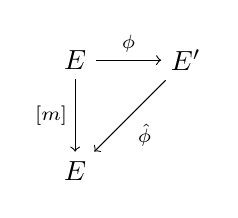
\begin{tikzpicture}[node distance=4em]
      \node(E1){$E$}; 
      \node(E2)[below of=E1]{$E$};
      \node(E')[right of=E1]{$E'$};
      \scriptsize
      \path[->] (E1) edge node[auto]{$\phi$} (E');
      \path[->] (E1) edge node[auto,swap]{$[m]$} (E2);
      \path[->] (E') edge node[auto]{$\hat{\phi}$} (E2);
    \end{tikzpicture}
  \end{center}

  \begin{itemize}
  \item \emph{$\hat\phi$} is called the \alert{dual isogeny},
    \emph{$\deg \phi = \deg \hat{\phi} = m$}.
  \item \emph{$\hat{\hat{\phi}} = \phi$}.
  \end{itemize}
  
  An obvious \textbf{corollary:} \emph{$\phi(E[m]) = \ker\hat\phi$}.
\end{frame}

%%

\begin{frame}
  \frametitle{Computational isogenies}
  
  \emph{In practice:} an isogeny $\phi$ is just a rational fraction (or maybe two)
  
  \alert{\[\frac{N(x)}{D(x)} = \frac{x^n + \cdots + n_1x +
      n_0}{x^{n-1} + \cdots + d_1x + d_0} \in k(x),\qquad\text{with }
    n=\deg\phi,\]}
  
  and $D(x)$ vanishes on $\ker\phi$.

  \begin{block}{The explicit isogeny problem}
    \begin{description}
    \item[Input:] A \textit{description} of the isogeny (e.g, its kernel).
    \item[Output:] The curve \emph{$E/H$} and the rational fraction \emph{$N/D$}.
    \item[Lower bound:] $\Omega(n)$.
    \end{description}
  \end{block}

  \begin{block}{The isogeny evaluation problem}
    \begin{description}
    \item[Input:] A \textit{description} of the isogeny \emph{$\phi$},
      a point \emph{$P\in E(k)$}.
    \item[Output:] The curve \emph{$E/H$} and \emph{$\phi(P)$}.
    \end{description}
  \end{block}
\end{frame}

%%

\begin{frame}
  \frametitle{The endomorphism ring}
  
  \begin{itemize}
  \item An \emph{endomorphism} is an isogeny \emph{$\phi:E\to E$}.
  \item The endomorphisms form a ring denoted \emph{$\End_k(E)$}.
  \end{itemize}

  \begin{theorem}
    \alert{$\Q\otimes\End_{\bar{k}}(E)$} is isomorphic to one of the
    following
    \begin{description}
    \item[ordinary case:] \alert{$\Q$} (only possible if $\chr k=0$),
    \item[ordinary case (complex multiplication):] an \alert{imaginary quadratic field},
    \item[supersingular case:] a \alert{quaternion algebra} (only possible if $\chr k\ne0$).
    \end{description}
  \end{theorem}

  \begin{corollary}
    \alert{$\End(E)$} is isomorphic to an \textit{order} 
    $\alert{\O}\subset\Q\otimes\End(E)$.
  \end{corollary}
\end{frame}

%%

\begin{frame}
  \frametitle{Isogeny walks}

  \begin{theorem}
    Two elliptic curves $E,E'$ are isogenous if and only if
    \[\emph{\Q\otimes\End(E) \simeq \Q\otimes\End(E')}.\]
  \end{theorem}

  \emph{Example:} Finite field, ordinary case

  \begin{center}
    Nice picture goes here
  \end{center}
\end{frame}

%%

\begin{frame}
  \frametitle{Isogeny walks}

  \begin{block}{Ramanujan properties}
    \begin{itemize}
    \item For any prime \emph{$\ell$}, the graph $G_\ell$ of
      \emph{$\ell$-isogenies} is an \emph{$\ell+1$-regular} graph.
    \item For any subset $S\subset G_\ell$, a random walk of length at
      least \[\emph{\sim\frac{2|G_\ell|}{\sqrt{|S|}}}\] hits $S$ with
      probability at least \emph{$|S|/2|G|$}.
    \end{itemize}
  \end{block}
\end{frame}

%%

\begin{frame}
  \frametitle{The class group}
  
  Let $E$ have complex multiplication and let $\O = \End(E)$. Define

  \begin{itemize}
  \item $\mathcal{I}(\O)$, the group of \emph{invertible fractional ideals},
  \item $\mathcal{P}(\O)$, the group of \emph{principal ideals} (i.e., real
    ideals),
  \end{itemize}
  
  \begin{definition}[The class group]
    The \alert{class group} of $\O$ is \[\alert{\Cl(\O) =
      \mathcal{I}(\O)/\mathcal{P}(O)}.\]
  \end{definition}

  \begin{itemize}
  \item It is a finite group.
  \item It arises as the Galois group of an abelian extension of
    $\Q\otimes\O$.
  \end{itemize}
\end{frame}

%%

\begin{frame}
  \frametitle{The action of the class group}
  
  \begin{definition}
    Let
    \begin{itemize}
    \item \emph{$\a$} be a fractional ideal of $\O$;
    \item \emph{$E[\a]$} be the the subgroup of $E(\bar{k})$
      annihilated by $\a$;
    \item \emph{$\phi:E\to E/E[\a]$}.
    \end{itemize}
    Then \emph{$\deg\phi = \mathcal{N}(\a)$}. We denote by \alert{$\ast$} the
    action on the set of elliptic curves.
    \[\alert{\a\ast j(E) = j(E/E[\a])}.\]
  \end{definition}

  \begin{theorem}
    The action $\ast$ \emph{factors through $\Cl(\O)$}. It is faithful
    and transitive.
  \end{theorem}
\end{frame}

%%

\begin{frame}
  \frametitle{The action of the class group}

  \emph{Example:} Let \emph{$\a = m\O$}, the ideal corresponding to
  multiplication by $m$. Then
  \begin{itemize}
  \item $\deg\phi = \mathcal{N}(m\O) = m^2$,
  \item $E[\a] = E[m]$,
  \item $m\O \in \mathcal{P}(\O)$,
  \item $m\O \equiv 1 \in \Cl(\O)$.
  \item $\a\ast j(E) = j(E)$.
  \end{itemize}
\end{frame}

%%

\begin{frame}
  \frametitle{Diffie-Hellman key exchange}
  
  Let \emph{$G=\cyc{g}$} be a cyclic group of prime order $p$.

  \begin{center}
    \begin{tikzpicture}
      \Large
      \node[matrix of math nodes, ampersand replacement=\&, column sep=1cm, row sep=1cm] (diagram) {
        \& |(1)| g \\
        |(a)| g^a \& \& |(b)| g^b\\
        \& |(ab)| g^{ab}\\
      };
      \small
      \path[->] (1) edge node[auto,swap]{$a$} (a);
      \path[->] (1) edge node[auto]{$b$} (b);
      \path[->] (a) edge node[auto,swap]{$b$} (ab);
      \path[->] (b) edge node[auto]{$a$} (ab);
    \end{tikzpicture}
  \end{center}

  \emph{Group action:} \alert{$\Z/p\Z$}  over \alert{$G$}.
\end{frame}

%%

\begin{frame}
  \frametitle{DH-like key exchange based on (semi)-group actions}
  
  Let \emph{$G$} be an abelian group acting (faithfully and
  transitively) on a set $\emph{X}$.

  \begin{center}
    \begin{tikzpicture}
      \Large
      \node[matrix of math nodes, ampersand replacement=\&, column sep=0cm, row sep=1cm] (diagram) {
        \& |(1)| x_0 \\
        |(a)| g\cdot x_0 \& \& |(b)| h\cdot x_0\\
        \& |(ab)| gh\cdot x_0 = hg\cdot x_0\\
      };
      \small
      \path[->] (1) edge node[auto,swap]{$g$} (a);
      \path[->] (1) edge node[auto]{$h$} (b);
      \path[->] (a) edge node[auto,swap]{$h$} (ab);
      \path[->] (b) edge node[auto]{$g$} (ab);
    \end{tikzpicture}
  \end{center}
\end{frame}

%%

\begin{frame}
  \frametitle{Hidden Subgroup Problem}
  
  Let \emph{$G$} be a group, \emph{$X$} a set and \emph{$f:G\to X$}.
  We say that $f$ \emph{hides} a subgroup \emph{$H\subset G$} if
  \[\alert{f(g_1) = f(g_2) \Leftrightarrow g_1H = g_2H}.\]

  \begin{definition}[Hidden Subgroup Problem (HSP)]
    \begin{description}
    \item[Input:] $G,X$ as above,  an oracle computing $f$.
    \item[Output:] generators of $H$.
    \end{description}
  \end{definition}

  \begin{theorem}[Schorr, Josza]
    If $G$ is abelian, then
    \begin{itemize}
    \item \alert{$\text{HSP}\in\text{poly}_\text{BQP}(\log|G|)$},
    \item using \alert{$\text{poly}(\log|G|)$} queries to the oracle.
    \end{itemize}
  \end{theorem}
\end{frame}

%%

\begin{frame}
  \frametitle{Discrete logarithm $\to$ HSP}

  Let \emph{$G=\cyc{g}$} of order \emph{$p$}, and let
  \emph{$h=g^s$}. Define

  \begin{equation*}
    \begin{aligned}
      f : (\Z/p\Z)^2 &\to G\\
      (a,b) &\mapsto g^ah^b = g^{a+sb}
    \end{aligned}
  \end{equation*}

  \emph{Remark:} A collision in $f$ uncovers the secret $s$, like in
  Pollard's Rho.

  \begin{block}{The reduction}
    \begin{itemize}
    \item $f$ is a group morphism;
    \item $\alert{\ker f = \cyc{(s,-1)}} \simeq \Z/p\Z$.
    \end{itemize}
    Hence $f$ \emph{hides} the secret $\cyc{(s,-1)}$.
  \end{block}

  \emph{Consequence:} Diffie-Hellman is broken by quantum computers
\end{frame}

%%

\begin{frame}
  \frametitle{The Hidden Shift Problem}
  
  The security of DH-like schemes based on group actions depends on

  \begin{definition}[(Semi)group Action Problem (SAP)]
    \begin{description}
    \item[Input:] A (semi)group \emph{$G$}, a set \emph{$X$}, elements
      \emph{$x,y\in X$}.
    \item[Output:] Find \emph{$s\in G$} such that \emph{$y=s\cdot x$}.
    \end{description}
  \end{definition}

  \begin{definition}[Hidden Shift Problem (HShP)]
    \begin{description}
    \item[Input:] \alert{$f_0,f_1:G\to X$} two oracles such that
      \alert{$f_1(g) = f_0(gs)$}.
    \item[Outpu:] The secret \alert{$s\in G$}.
    \end{description}
  \end{definition}
\end{frame}

%%

\begin{frame}
  \frametitle{The Hidden Shift Problem}
  
  \begin{block}{Reductions}
    \begin{itemize}
    \item \emph{SAP $\to$ HShP} (evident).
    \item \emph{HShP $\to$ non-abelian HSP} for the dihedral group
      $G\ltimes\Z/2\Z$.
    \end{itemize}
  \end{block}

  \begin{block}{Quantum algorithms:}
    \begin{description}
    \item[Kuperberg:] \alert{$2^{O(\sqrt{\log|G|})}$} quantum time and space
      and query complexity.
    \item[Regev:] \alert{$L_{|G|}(\frac{1}{2},\sqrt{2})$} quantum
      time and query complexity, \alert{$\text{poly}(\log(|G|)$} quantum
      space.
    \end{description}
  \end{block}

  \emph{Remark (Regev):} certain lattice-based cryptosystems are also
  vulnerable to the HSP for dihedral groups.
\end{frame}

%%

\begin{frame}
  \frametitle{Rostovstev and Stolbunov's key exchange}
  
  \emph{Public data:}
  \begin{itemize}
  \item \alert{$E/\F_p$ ordinary elliptic curve} with complex multiplication
    field $\mathbb{K}$,
  \item \alert{primes $\ell_1,\ell_2$} not dividing $\mathrm{Disc}(E)$ and
    s.t. $\left(\frac{D_\mathbb{K}}{\ell_i}\right)=1$.
  \item A \textit{direction} on the isogeny graph (a Frobenius eigenvalue).
  \end{itemize}

  \emph{Secret data:}  \alert{Random walks $\a,\b$} in the
  $\ell_i$-isogeny graphs.
  
  \begin{center}
    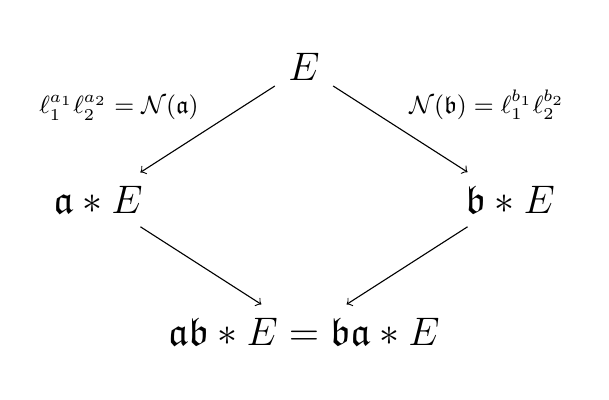
\begin{tikzpicture}
      \Large
      \node[matrix of math nodes, ampersand replacement=\&, column sep=0cm, row sep=1cm] (diagram) {
        \& |(1)| E \\
        |(a)| \a\ast E \& \& |(b)| \b\ast E\\
        \& |(ab)| \a\b\ast E = \b\a\ast E\\
      };
      \small
      \path[->] (1) edge node[auto,swap]{$\ell_1^{a_1}\ell_2^{a_2}=\mathcal{N}(\a)$} (a);
      \path[->] (1) edge node[auto]{$\mathcal{N}(\b)=\ell_1^{b_1}\ell_2^{b_2}$} (b);
      \path[->] (a) edge (ab);
      \path[->] (b) edge (ab);
    \end{tikzpicture}
  \end{center}
\end{frame}

%%

\begin{frame}
  \frametitle{Rostovstev and Stolbunov's key exchange}

  \begin{center}
    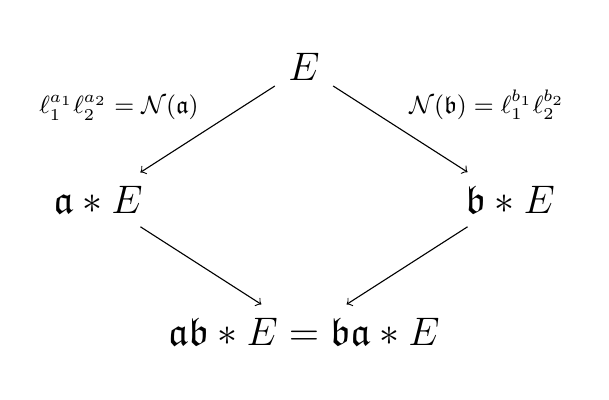
\begin{tikzpicture}
      \Large
      \node[matrix of math nodes, ampersand replacement=\&, column sep=0cm, row sep=1cm] (diagram) {
        \& |(1)| E \\
        |(a)| \a\ast E \& \& |(b)| \b\ast E\\
        \& |(ab)| \a\b\ast E = \b\a\ast E\\
      };
      \small
      \path[->] (1) edge node[auto,swap]{$\ell_1^{a_1}\ell_2^{a_2}=\mathcal{N}(\a)$} (a);
      \path[->] (1) edge node[auto]{$\mathcal{N}(\b)=\ell_1^{b_1}\ell_2^{b_2}$} (b);
      \path[->] (a) edge (ab);
      \path[->] (b) edge (ab);
    \end{tikzpicture}
  \end{center}

  \begin{description}
  \item[Key generation:] compose small degree
    isogenies\\\alert{polynomial in the lenght of the random walk}.
  \item[Attack:] find an isogeny between two curves\\\alert{polynomial
      in the degree}.
  \item[Quantum (Childs-Jao-Soukharev):] HShP + isogeny
    evaluation\\\alert{subexponential in the length of the walk}.
  \end{description}
\end{frame}

%%

\begin{frame}
  \frametitle{Supersingular curves}

  \emph{$\Q\otimes\End(E)$} is a quaternion algebra (it is non-commutative)

  \begin{block}{Propositions}
    \begin{itemize}
    \item Every supersingular curve is defined over \alert{$\F_{p^2}$}.
    \item There are $g(X(0)) \sim\alert{\frac{p+1}{12}}$ supersingular curves
      up to isomorphism.
    \item $\alert{E(\F_{p^2}) \simeq (\Z/(p+1)\Z)^2}\;$ (up to twist).
    \item There is an \alert{unique isogeny class} of supersingular
      curves.
    \end{itemize}
  \end{block}

  Constructing supersingular curves is easy:
  \begin{itemize}
  \item Find a discriminant $D$ such that $\left(\frac{D}{p}\right)=-1$;
  \item Factor the Hilbert class polynomial $H_D$ in $\F_{p^2}$;
  \item Perform a random walk in the isogeny graph (to improve randomness).
  \end{itemize}
\end{frame}

%%

\begin{frame}
  \frametitle{Good and bad news}
  
  \begin{description}
  \item[Good news:] On supersingular curves there is no action of a
    commutative class group.
  \item[Bad news:] On supersingular curves there is no action of a
    commutative class group.
  \end{description}

  \alert{New idea:} Use isogenies to hide disjoint subgroups
  \emph{$G,H\subset E$}

  \begin{center}
    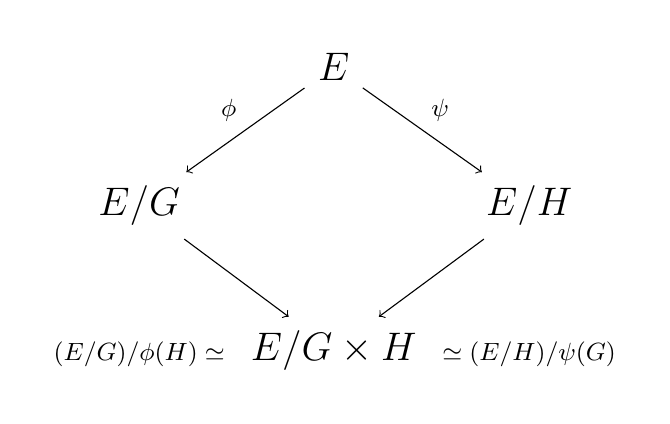
\begin{tikzpicture}
      \Large
      \node[matrix of nodes, ampersand replacement=\&, column sep=0cm, row sep=1cm] (diagram) {
        \& |(1)| $E$ \\
        |(a)| $E/G$ \& \& |(b)| $E/H$\\
        \small $(E/G)/\phi(H) \simeq$ \& |(ab)|  $E/G\times H$ \& \small $\simeq (E/H)/\psi(G)$\\
      };
      \small
      \path[->] (1) edge node[auto,swap]{$\phi$} (a);
      \path[->] (1) edge node[auto]{$\psi$} (b);
      \path[->] (a) edge (ab);
      \path[->] (b) edge (ab);
    \end{tikzpicture}
  \end{center}
\end{frame}

%%

\begin{frame}
  \frametitle{Three \textit{caveats} (and a half)}

  \begin{center}
    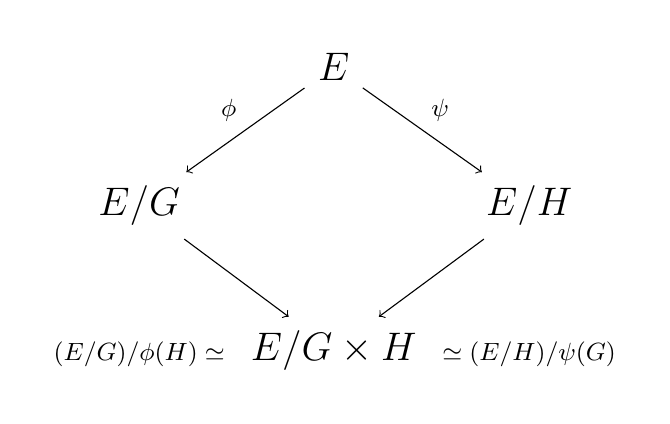
\begin{tikzpicture}
      \Large
      \node[matrix of nodes, ampersand replacement=\&, column sep=0cm, row sep=1cm] (diagram) {
        \& |(1)| $E$ \\
        |(a)| $E/G$ \& \& |(b)| $E/H$\\
        \small $(E/G)/\phi(H) \simeq$ \& |(ab)|  $E/G\times H$ \& \small $\simeq (E/H)/\psi(G)$\\
      };
      \small
      \path[->] (1) edge node[auto,swap]{$\phi$} (a);
      \path[->] (1) edge node[auto]{$\psi$} (b);
      \path[->] (a) edge (ab);
      \path[->] (b) edge (ab);
    \end{tikzpicture}
  \end{center}  

  \begin{itemize}
  \item[1] \alert{Additional information} must be passed to compute
    \alert{$\phi(H)$}.
  \item[2] $\phi$ \alert{hides a subgroup}. An attacker with oracle
    access to $\phi$ can use HSP.
  \item[2$\frac{1}{2}$] Furthermore, it is easy to show that an
    attacker with oracle access to $\phi$ can break the scheme
    classically.
  \item[3] For generic $G$, evaluating $\phi$ is \alert{polynomial in
      $|G|$}.
  \end{itemize}
\end{frame}

%%

\begin{frame}
  \frametitle{Our proposal}

  \begin{columns}
    \begin{column}{0.4\textwidth}
      \begin{block}{}
        \emph{Public data:}
        \begin{itemize}
          \setlength{\itemsep}{1.5ex}
        \item Prime \alert{$p$} such that \alert{$p+1 = \ell_A^a\ell_B^b$};
        \item Supersingular curve \alert{$E\simeq (\Z/(p+1)\Z)^2$};
        \item \alert{$E[\ell_B^b] = \cyc{P_A,Q_A}$};
        \item \alert{$E[\ell_A^a] = \cyc{P_B,Q_B}$}.
        \end{itemize}

        \emph{Secret data:}
        \begin{itemize}
          \setlength{\itemsep}{1.5ex}
        \item \alert{$R_A = m_AP_A + n_AQ_A$},
        \item \alert{$R_B = m_BP_B + n_BQ_B$},
        \end{itemize}
      \end{block}
    \end{column}
    \begin{column}{0.58\textwidth}
      \begin{center}
        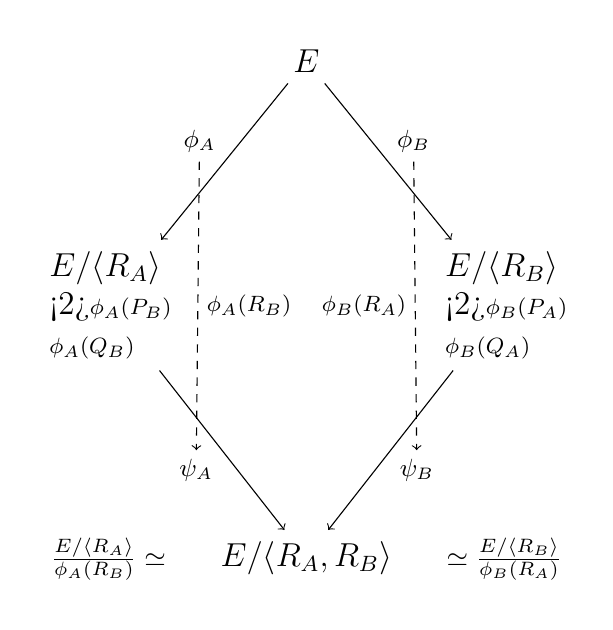
\begin{tikzpicture}
          \large
          \node[matrix of nodes, ampersand replacement=\&, column sep=4mm, row sep=2cm] (diagram) {
            \& |(1)| $E$ \\
            |(a)| \parbox{1.5cm}{$E/\cyc{R_A}$\\\uncover<2>{{\footnotesize $\phi_A(P_B)\\\phi_A(Q_B)$}}} \& \&
            |(b)| \parbox{1.5cm}{$E/\cyc{R_B}$\\\uncover<2>{{\footnotesize $\phi_B(P_A)\\\phi_B(Q_A)$}}}\\
            \normalsize $\frac{E/\cyc{R_A}}{\alert{\phi_A(R_B)}} \simeq$ \&
            |(ab)|  $E/\cyc{R_A,R_B}$ \&
            \normalsize $\simeq \frac{E/\cyc{R_B}}{\alert{\phi_B(R_A)}}$\\
          };
          \small
          \path[->] (1) edge node[auto,swap](phia) {$\phi_A$} (a);
          \path[->] (1) edge node[auto](phib) {$\phi_B$} (b);
          \path[->] (a) edge node[auto,swap](psia){$\psi_A$} (ab);
          \path[->] (b) edge node[auto](psib){$\psi_B$} (ab);
          \uncover<2>{\alert{\path[dashed,->] (phia) edge node[auto]{\footnotesize $\phi_A(R_B)$} (psia);}}
          \uncover<2>{\alert{\path[dashed,->] (phib) edge node[auto,swap]{\footnotesize $\phi_B(R_A)$} (psib);}}
        \end{tikzpicture}
      \end{center}  
    \end{column}
  \end{columns}
\end{frame}

%%

\begin{frame}
  \frametitle{Generic attacks}
  
  \emph{Problem:} Given \emph{$E,E'$}, isogenous of degree
  \emph{$\ell^n$}, find \emph{$\phi:E\to E'$}.

  \begin{center}
    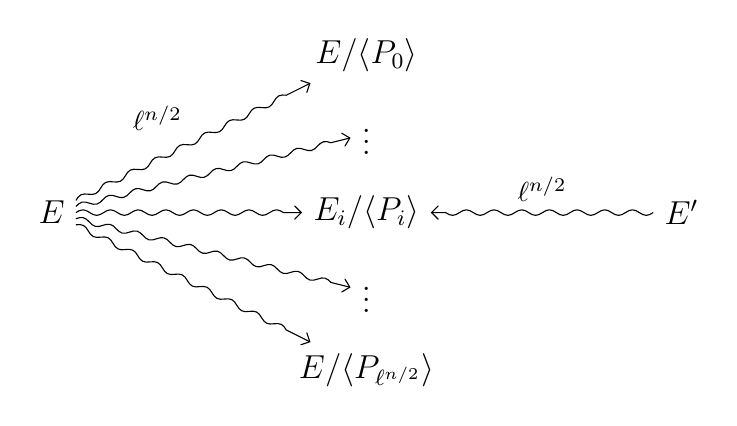
\begin{tikzpicture}[xscale=4,coils/.style={-angle 90,decorate,decoration={coil,aspect=0,amplitude=1pt}}]
      \large
      \draw (0,2) node(E) {$E$};

      \draw (1,4) node(E1) {$E/\cyc{P_0}$};
      \draw (1,2) node(Ei) {$E_i/\cyc{P_i}$};
      \draw (1,0) node(En) {$E/\cyc{P_{\ell^{n/2}}}$};
      \draw (1,3) node(dots1) {$\vdots$};
      \draw (1,1) node(dots2) {$\vdots$};

      \draw (2,2) node(E') {$E'$};

      \draw (E) edge[coils] node[auto] {\normalsize$\ell^{n/2}$} (E1);
      \draw (E) edge[coils] (Ei);
      \draw (E) edge[coils] (En);
      \draw (E) edge[coils] (dots1);
      \draw (E) edge[coils] (dots2);

      \draw (E') edge[coils] node[auto,swap] {\normalsize$\ell^{n/2}$} (Ei);
    \end{tikzpicture}
  \end{center}

  \begin{itemize}
  \item With high probability $\phi$ is the unique collision (or \textit{claw}).
  \item A \emph{quantum claw finding} algorithm solves the problem in
    $\alert{O(\ell^{n/3})}$ (Tani).
  \end{itemize}

\end{frame}

%%

\begin{frame}
  \frametitle{Our recommended parameters}
  
  \begin{itemize}
  \item For efficiency chose $p$ such that \alert{$p+1 = 2^a3^b$}.
  \item For classical $n$-bit security, choose \alert{$2^a\sim3^b\sim2^{2n}$}, hence \alert{$p\sim2^{4n}$}.
  \item For quantum $n$-bit security, choose \alert{$2^a\sim3^b\sim2^{3n}$}, hence \alert{$p\sim2^{6n}$}.
  \end{itemize}

  \begin{block}{Practical optimizations:}
    \begin{itemize}
    \item $-1$ is a quadratic non-residue: \alert{$\F_{p^2}\simeq\F_p[X]/(X+1)$}.
    \item $E$ (or its twist) has a $4$-torsion point: it has an
      \alert{Edwards} and a \alert{Montgomery} form.
    \item Other optimizations in the next slides.
    \end{itemize}
  \end{block}

\end{frame}

%%

\begin{frame}
  \frametitle{Analysis of the key exchange}
  
  \begin{block}{Round 1}
    \begin{itemize}
    \item Pick random \alert{$m,n\in\Z$};
    \item Compute \alert{$R = mP + nQ$};
    \item Compute \alert{$\phi : E \to E/\cyc{R}$};
    \item Evaluate \alert{$\phi(S), \phi(T)$} for some points $S,T$.
    \end{itemize}
  \end{block}
  
  \begin{block}{Round 2}
    \begin{itemize}
    \item Compute \alert{$R' = mP' + nQ'$};
    \item Compute \alert{$\psi : E \to E/\cyc{R'}$};
    \end{itemize}
  \end{block}
\end{frame}

%%

\begin{frame}
  \frametitle{Analysis of the key exchange: $R=mP+nQ$}

  \begin{itemize}
  \item To compute \emph{$\phi:E\to E/\cyc{R}$} only a
    \alert{genarator of $\cyc{R}$} is needed.
  \item We can compute \alert{$R'=P + m^{-1}nQ$} instead.
  \end{itemize}

  \begin{block}{Solution 1}
    \begin{itemize}
    \item Use Edwards coordinates.
    \item \emph{Drawback:} vulnerable to SPA.
    \end{itemize}
  \end{block}
  
  \begin{block}{Solution 2}
    \begin{itemize}
    \item Use Montgomery ladders.
    \item \emph{Security:} resistant to SPA.
    \item \emph{Efficiency:} we give a \alert{4-point Montgomery
        ladder} compatible with \alert{differential addition} in
      Montgomery coordinates. \emph{Nearly as efficient} as solution
      1.
    \end{itemize}
  \end{block}
\end{frame}

%%

\begin{frame}
  \frametitle{Analysis of the key exchange: $\phi:E\to E/\cyc{R}$}
  
  \alert{$\ord(R)=\ell^a$} and \alert{$\phi = \phi_0 \circ \phi_1 \circ \cdots
    \circ \phi_{a-1}$}, each of degree $\alert{\ell}$

  \begin{center}
  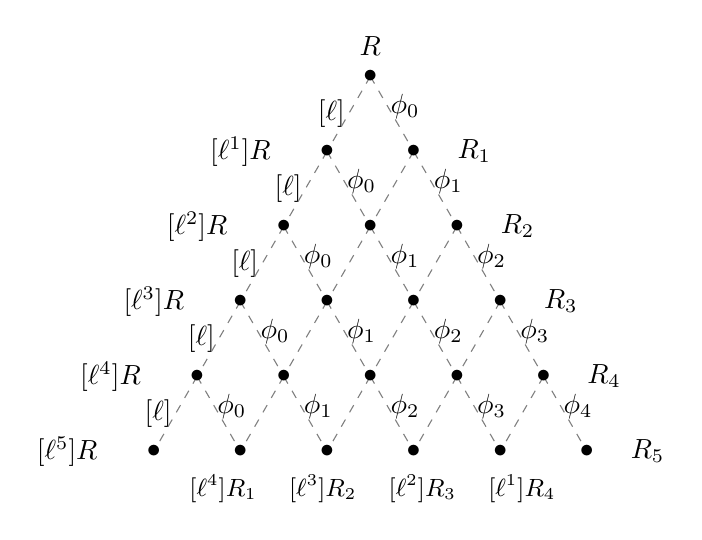
\begin{tikzpicture}[/triangle,scale=1.1]
    \def\n{5}
    \pgfmathtruncatemacro{\pn}{\n-1}
    

    \draw(-0.4,-0.2) node{$R$};

    \foreach \i in {1,...,\n} {
      \draw(\i,\i+0.7) node{$R_\i$};
    }
    \foreach \i in {1,...,\n} {
      \draw(\i,-1) node{$[\ell^\i]R$};
    }
    \foreach \i in {0,...,\pn} {
      \pgfmathtruncatemacro{\ii}{\pn-\i}
      \foreach \j in {0,...,\ii} {
        \draw(\i+\j+0.4,\i+0.6) node{$\phi_\i$};
      }
    }
    \foreach \i in {0,...,\pn} {
      \draw(\i+0.5,-0.2) node{$[\ell]$};
    }

    \foreach \i in {1,...,\pn} {
      \pgfmathtruncatemacro{\ii}{\n-\i}
      \draw(\n+0.5,1.15*\i-0.1) node{\alert{\small $[\ell^\ii]R_\i$}};
    }

    \foreach \i in {0,...,\pn} {
      \foreach \j in {0,...,\i} {
        \draw[gray,dashed]  (\i,\j) -- (\i+1,\j+1);
        \draw[gray,dashed]  (\i,\j) -- (\i+1,\j);
      }
    }

    \dottriangle[$\bullet$]{\n}
  \end{tikzpicture}
  \end{center}
  For each $i$, one needs to compute \alert{$[\ell^{e-i}]R_i$} in
  order to compute $\phi_i$.
\end{frame}

%%


\begin{frame}
  \frametitle{What's the best strategy?}

  \begin{figure}
    \centering
    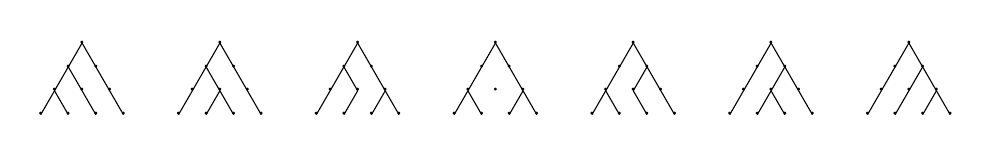
\begin{tikzpicture}[/triangle,scale=0.35]
      \def\n{3}
      \newlength{\shift}
      \setlength{\shift}{5cm}

      \foreach \k in {0,...,6} {
        \begin{scope}[xshift=\k\shift]
          \dottriangle[$\cdot$]{\n}
          \foreach \i in {1,...,\n} {
            \draw(\i-1,0) -- (\i,0);
          }
          \foreach \i in {1,...,\n} {
            \draw(\i-1,\i-1) -- (\i,\i);
          }
        \end{scope}
      }

      \begin{scope}
        \draw (1,0)--(2,1) (2,1)--(3,2) (2,0)--(3,1);
      \end{scope}

      \begin{scope}[xshift=\shift]
        \draw (1,0)--(2,1) (2,1)--(3,1) (2,1)--(3,2);
      \end{scope}

      \begin{scope}[xshift=2\shift]
        \draw (1,0)--(2,1) (2,1)--(3,1) (2,2)--(3,2);
      \end{scope}

      \begin{scope}[xshift=3\shift]
        \draw (2,0)--(3,1) (2,2)--(3,2);
      \end{scope}

      \begin{scope}[xshift=4\shift]
        \draw (1,1)--(2,1) (2,1)--(3,2) (2,0)--(3,1);
      \end{scope}

      \begin{scope}[xshift=5\shift]
        \draw (1,1)--(2,1) (2,1)--(3,2) (2,1)--(3,1);
      \end{scope}

      \begin{scope}[xshift=6\shift]
        \draw (1,1)--(2,1) (2,1)--(3,1) (2,2)--(3,2);
      \end{scope}
    \end{tikzpicture}
    \caption{The seven well formed strategies for $e=4$.}
  \end{figure}

  \begin{itemize}
  \item Right edges are \alert{$\ell$-isogeny evaluation};
  \item Left edges are \alert{multiplications by $\ell$} (about twice as expensive);
  \end{itemize}

  The best strategy can be \alert{precomputed} offline and
  \alert{hardcoded} in an embedded system.

  \begin{block}{}
    \emph{Funny fact:} strategies are in one-to-one correspondence with
    certain instances of Gelfand-Tsetlin polytopes [OEIS, Sequence
    A130715].
  \end{block}
\end{frame}


\begin{frame}
  \frametitle{What's the best strategy?}

  \begin{lemma}
    Strategies with \textit{zig-zags} can be straightened.
  \end{lemma}

  \begin{figure}
    \centering
    \begin{tikzpicture}[/triangle,scale=0.3]
      \def\n{3}
      \setlength{\shift}{5cm}

      \foreach \k in {0,...,1} {
        \begin{scope}[xshift=\k\shift]
          \dottriangle[$\cdot$]{\n}
          \foreach \i in {1,...,\n} {
            \draw(\i-1,0) -- (\i,0);
          }
          \foreach \i in {1,...,\n} {
            \draw(\i-1,\i-1) -- (\i,\i);
          }
        \end{scope}
      }

      \begin{scope}
        \draw (1,1)--(2,1) (2,1)--(3,2) (2,0)--(3,1);
      \end{scope}
      
      \begin{scope}[xshift=0.5\shift]
        \draw (2,1) node {$\to$};
      \end{scope}

      \begin{scope}[xshift=\shift]
        \draw (2,0)--(3,1) (2,2)--(3,2);      
      \end{scope}
    \end{tikzpicture}
  \end{figure}

  \begin{lemma}
    An optimal strategy is a binary tree. Its subtrees are optimal
    strategies.
  \end{lemma}

  \begin{corollary}
    Let \emph{$p,q$} be the costs of evaluating a \emph{left or right}
    edge respectively. Then the asymptotic cost of a strategy of
    height \emph{$n$} grows like $\alert{n\log_r n}$, where \emph{$r$}
    is the solution to the generalized Fibonacci
    equation \[\alert{1=r^{-p}+r^{-q}}.\]
  \end{corollary}
\end{frame}

%% 

\begin{frame}
\frametitle{Example}
\begin{figure}[t]
  \centering
  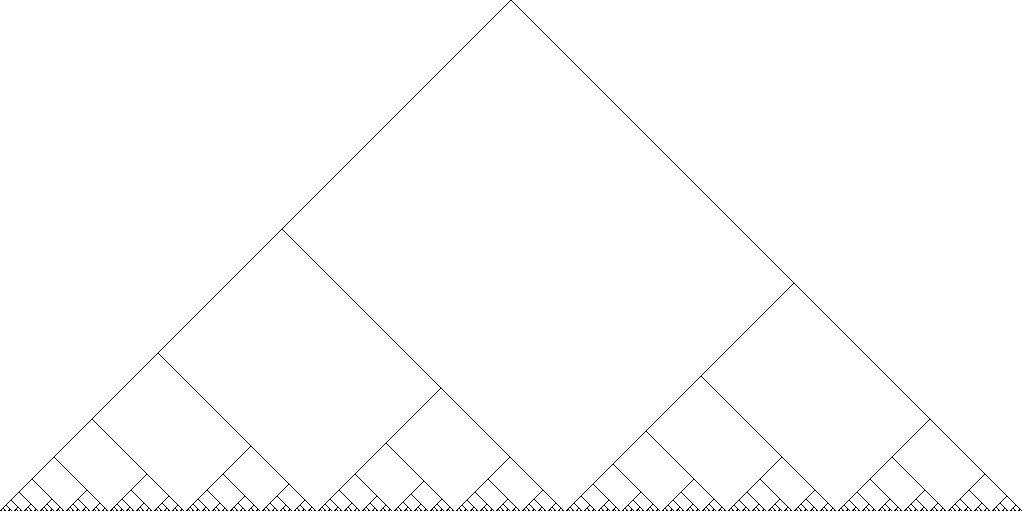
\includegraphics[width=\textwidth]{optimal.png}
  \caption{Optimal strategy for $e=512$, $\ell=2$.}
  \label{fig:optimal}
\end{figure}
\end{frame}

%% 

\begin{frame}
  \frametitle{Timings}
  
  \begin{block}{Reference implementation}
    Available at \alert{\url{http://www.prism.uvsq.fr/~dfl/}}
    \begin{itemize}
    \item C + GMP implementation of $\F_{p^2}$;
    \item C implementation of the key exchange;
    \item Cython interface to the key exchange and implementation of
      elliptic curves;
    \item Python + Sage script for parameter generation and strategy computation.
    \end{itemize}
  \end{block}

  \begin{center}
    \begin{tabular}{l r r r}
      \hline
      & 512 bits & 768 bits & 1024 bits\\
      \hline
      Alice round 1 & 29 ms & 66 ms & 123 ms \\
      Alice round 2 & 24 ms & 55 ms & 102 ms \\
      Bob round 1 & 37 ms & 86 ms & 163 ms \\
      Bob round 2 & 30 ms & 69 ms & 130 ms
    \end{tabular}
  \end{center}
\end{frame}

%%

\begin{frame}
  \frametitle{Conclusion}
  
  We have proposed a new candidate for \emph{post-quantum cryptography}.

  \begin{itemize}
  \item It is based on a \emph{new group theoretic construction} that
    does not seem to have been used before.
  \item It is based on well known objects for which a lot of good
    software already exists.
  \item It is reasonably \emph{fast}:
    \begin{itemize}
    \item More than 1000 times faster than Rostovstev and Stolbunov's
      system at the same (classical) security level.
    \item Running times comparable to pairing-based protocols.
    \end{itemize}
  \item Because of its novelty, more scrutiny is required to assess
    its security. In particular, it is not clear \emph{what mathematical
    assumptions} are needed to \emph{prove its security}.
  \end{itemize}
\end{frame}

\end{document}



% Local Variables:
% mode:flyspell
% ispell-local-dictionary:"american"
% mode:TeX-PDF
% mode:reftex
% End:
%
% LocalWords:  Isogeny abelian isogenies hyperelliptic supersingular Frobenius
% LocalWords:  isogenous


